\documentclass[../labs.tex]{subfiles}

\pagestyle{main}
\renewcommand{\leftmark}{Lab Report \thesection}
\setcounter{section}{4}

\begin{document}




\noindent Steven Labalme\\
9 February 2023\hfill
23 February 2023

\section{GCMS ANALYSIS OF BENZENE IN GASOLINE}
\begin{figure}[H]
    \centering
    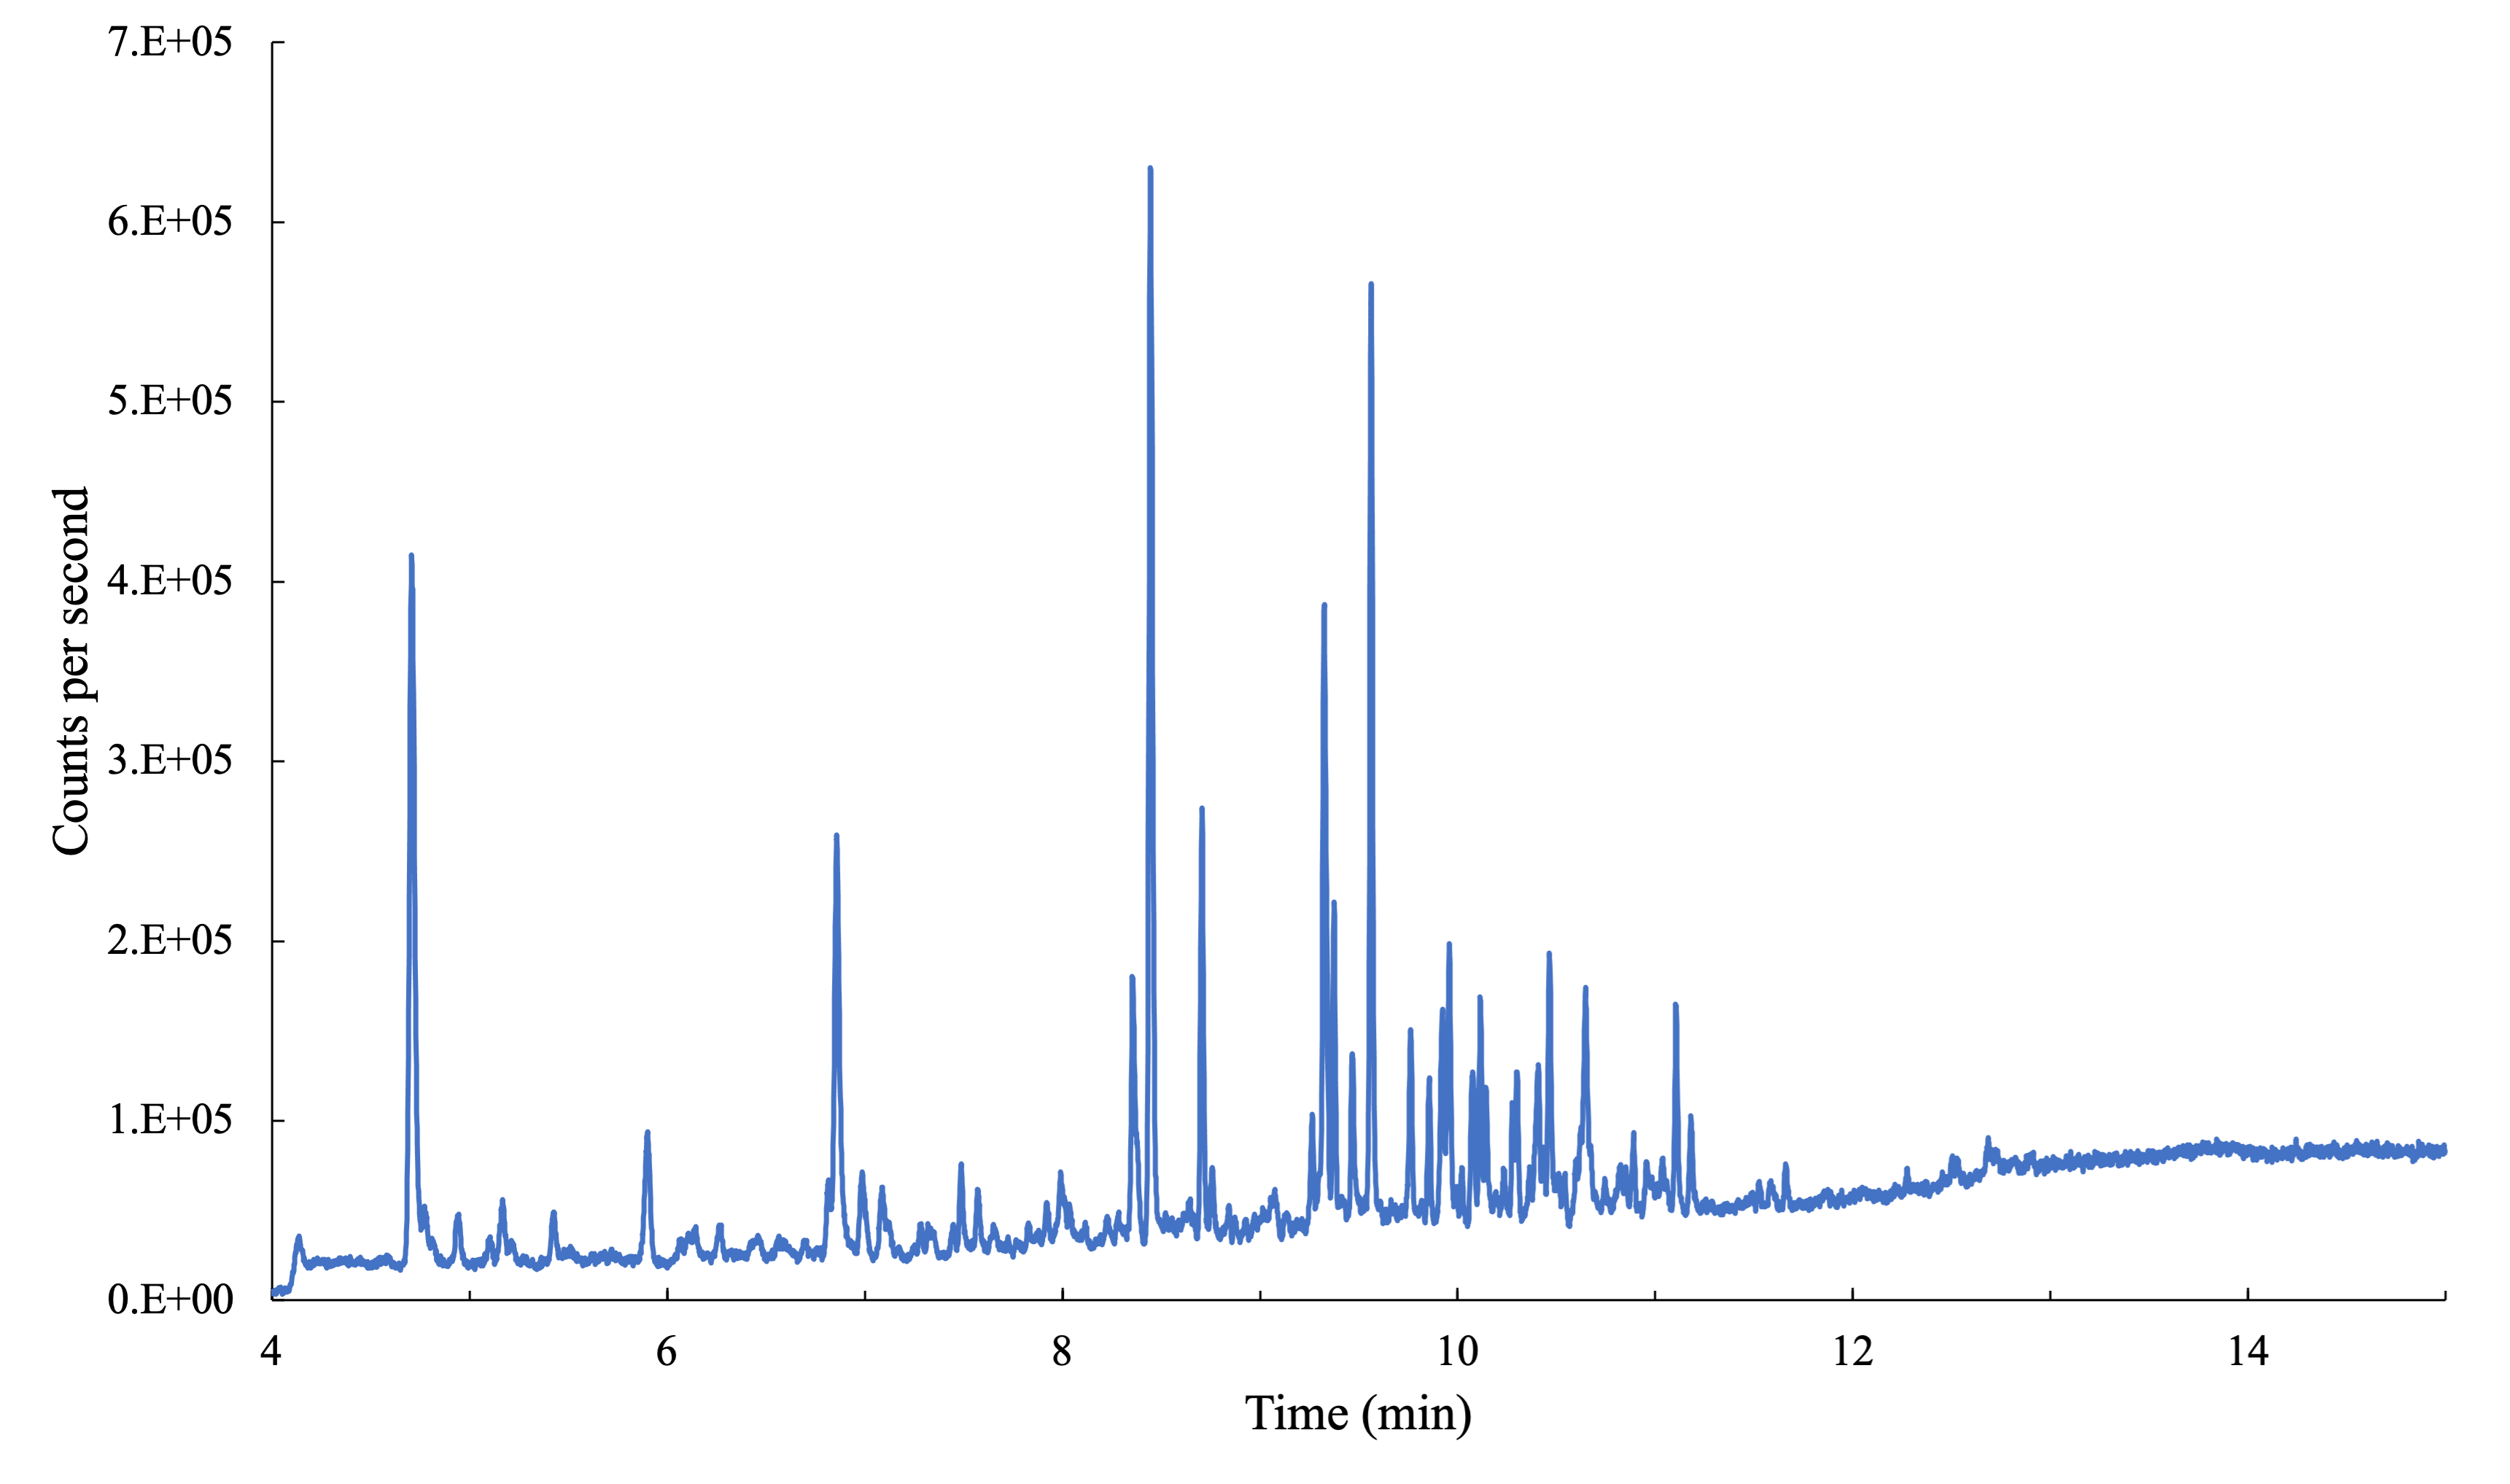
\includegraphics[width=0.95\linewidth]{lab4-TIC.png}
    \caption{Total ion chromatogram of diluted 87-gasoline in pentane.}
    \label{fig:TIC}
\end{figure}

\begin{figure}[H]
    \centering
    \begin{subfigure}[b]{0.49\linewidth}
        \centering
        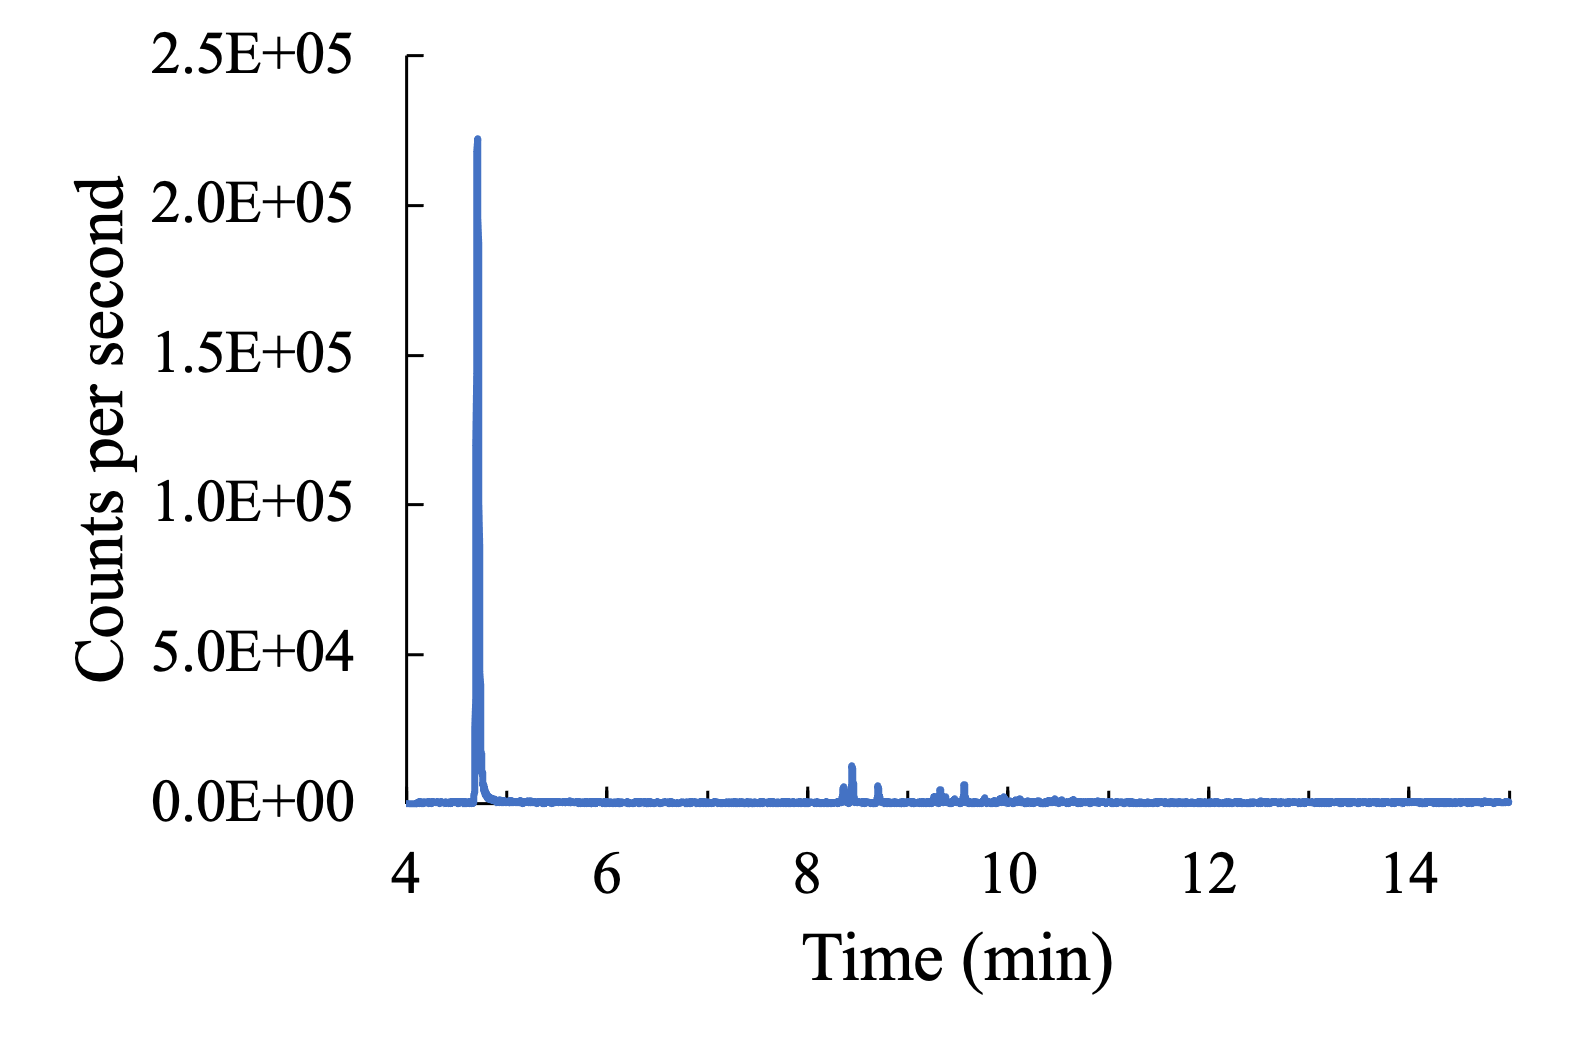
\includegraphics[width=0.9\linewidth]{lab4-BenzTolEICMSa.png}
        \caption{Benzene EIC.}
        \label{fig:BenzTolEICMSa}
    \end{subfigure}
    \begin{subfigure}[b]{0.49\linewidth}
        \centering
        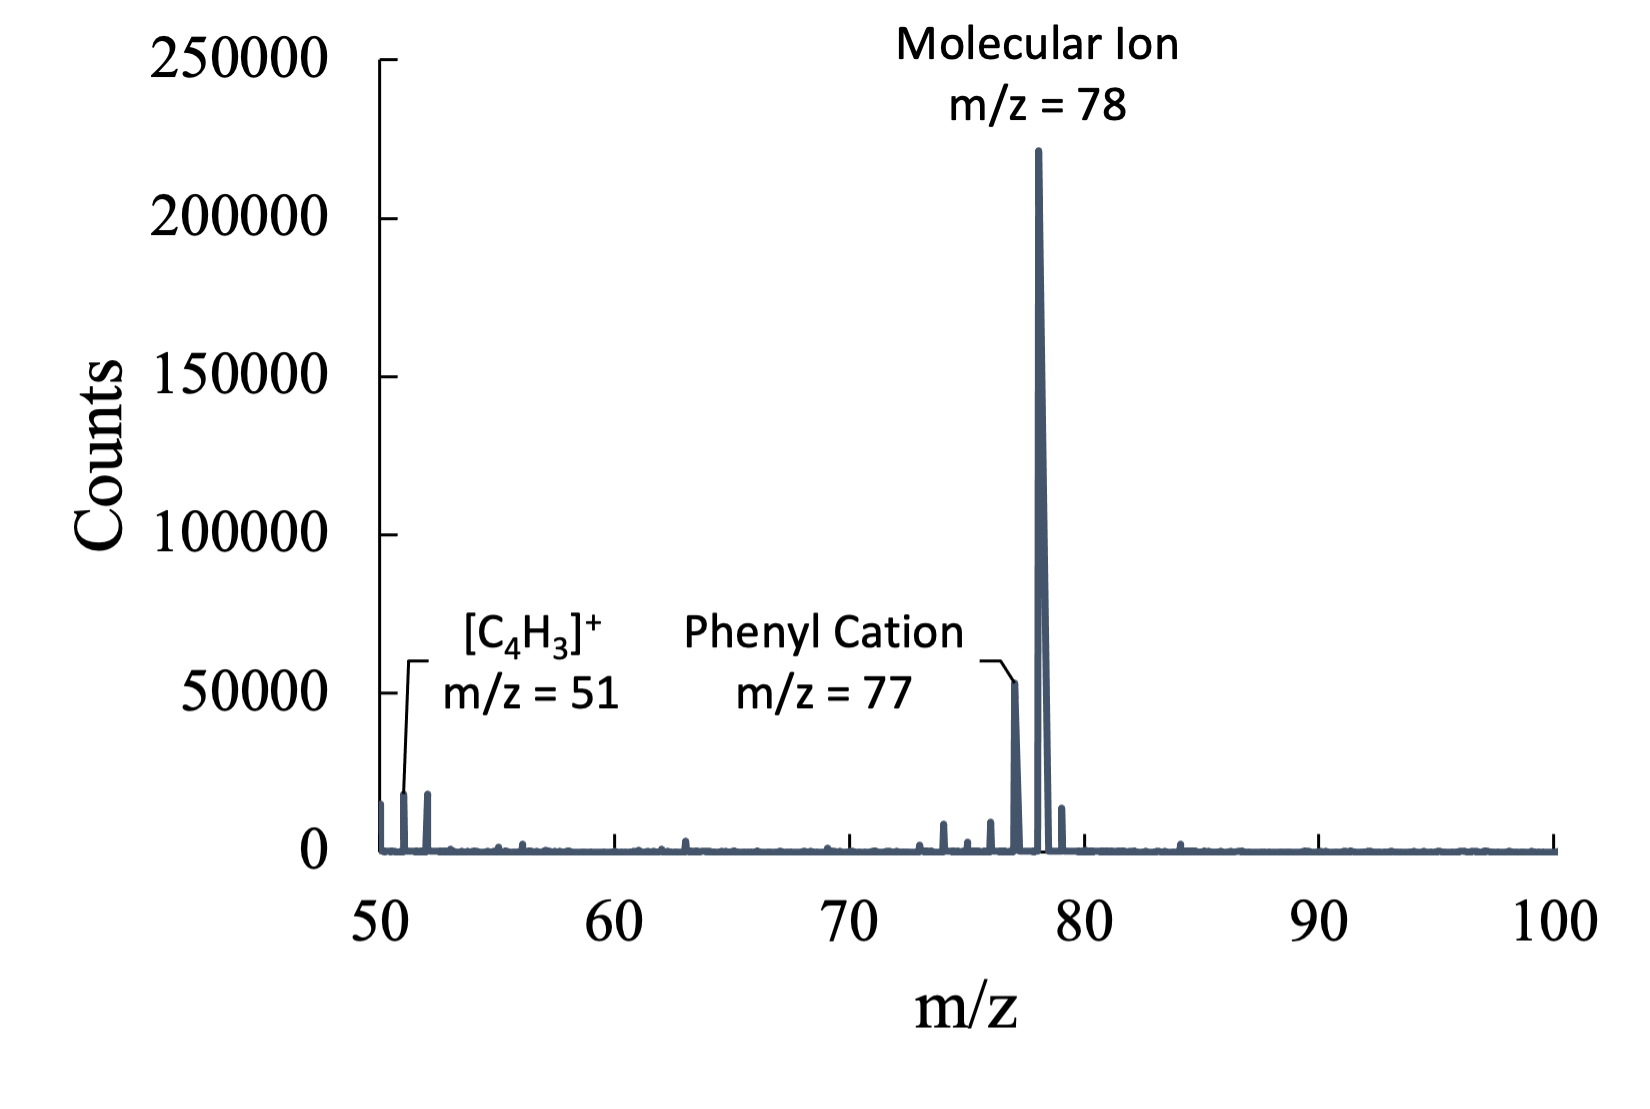
\includegraphics[width=0.9\linewidth]{lab4-BenzTolEICMSb.png}
        \caption{Benzene MS.}
        \label{fig:BenzTolEICMSb}
    \end{subfigure}\\[1em]
    \begin{subfigure}[b]{0.49\linewidth}
        \centering
        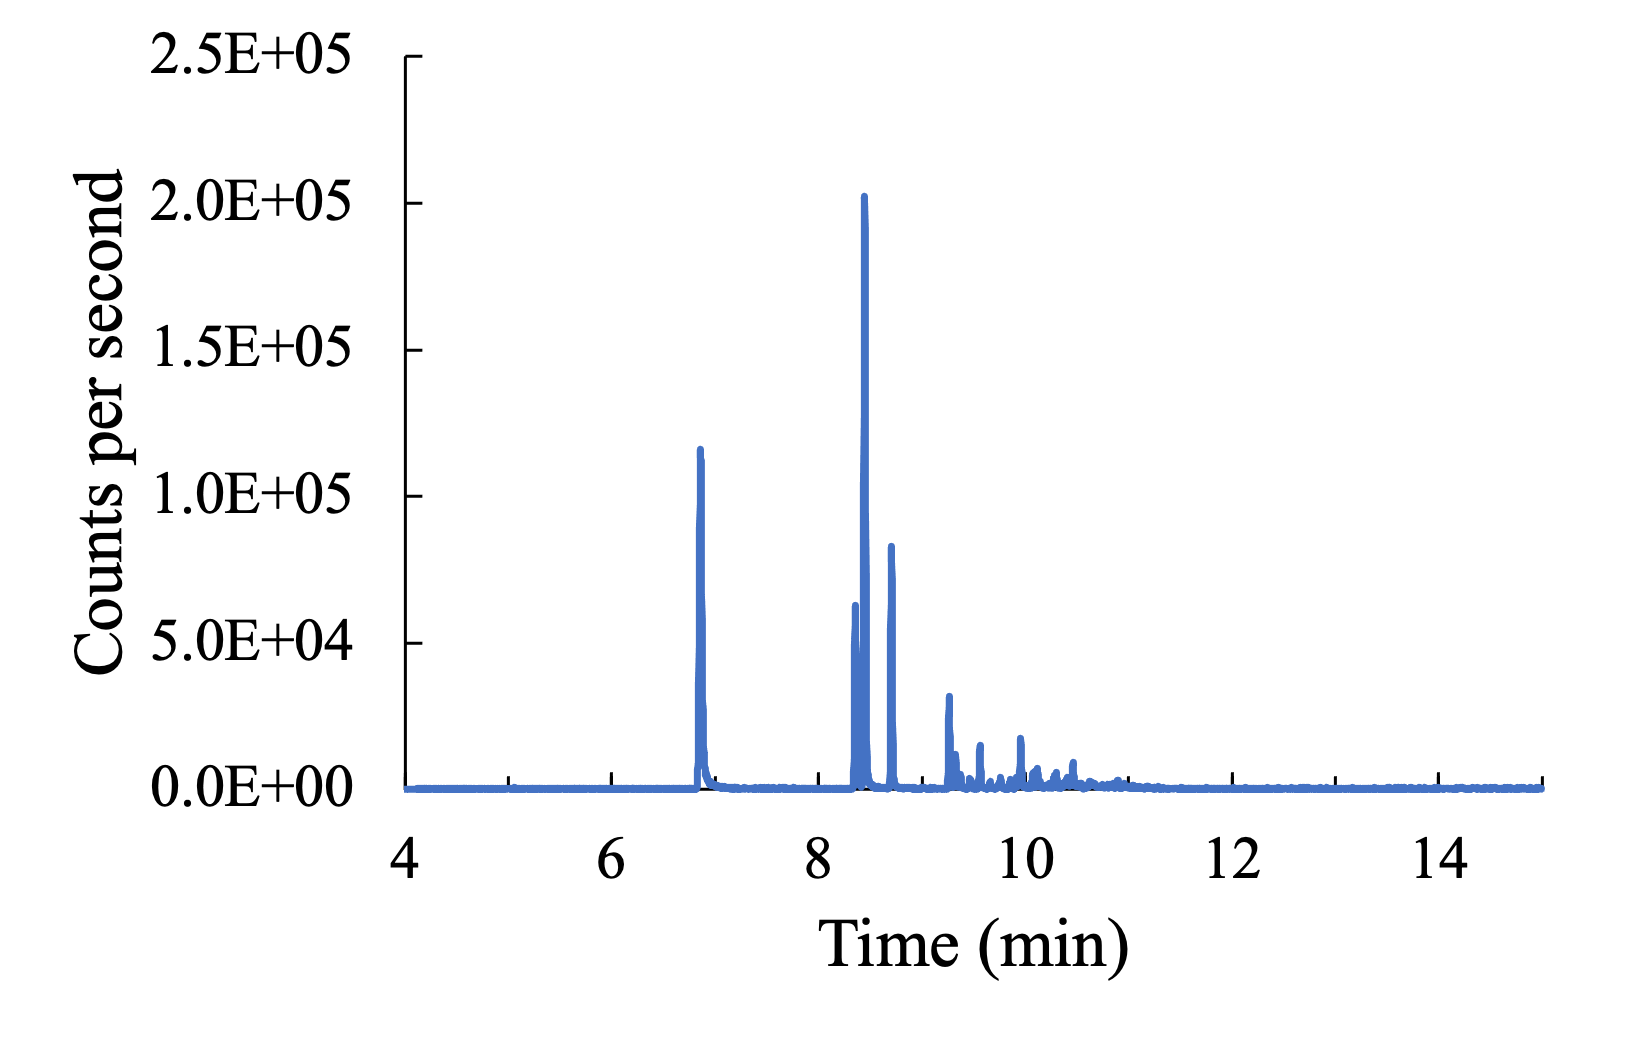
\includegraphics[width=0.9\linewidth]{lab4-BenzTolEICMSc.png}
        \caption{Toluene EIC.}
        \label{fig:BenzTolEICMSc}
    \end{subfigure}
    \begin{subfigure}[b]{0.49\linewidth}
        \centering
        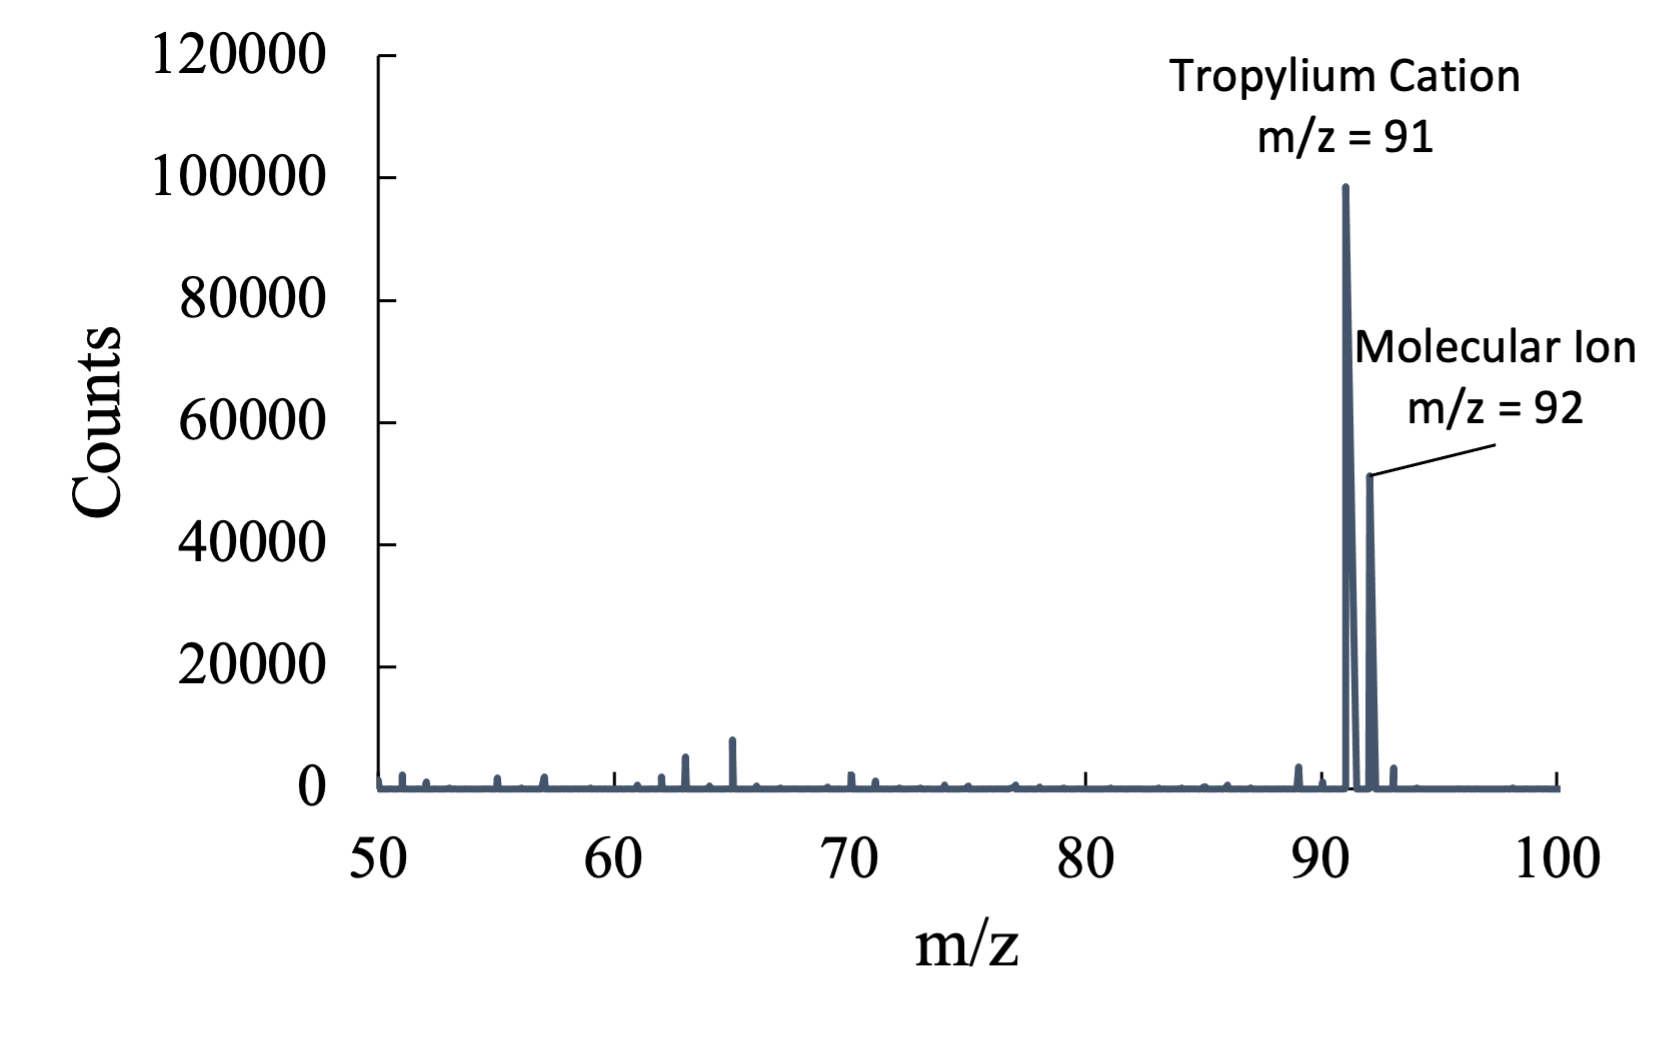
\includegraphics[width=0.9\linewidth]{lab4-BenzTolEICMSd.png}
        \caption{Toluene MS.}
        \label{fig:BenzTolEICMSd}
    \end{subfigure}
    \caption{Extracted ion chromatograms and extracted mass spectra for benzene and toluene.}
    \label{fig:BenzTolEICMS}
\end{figure}

\begin{figure}[H]
    \centering
    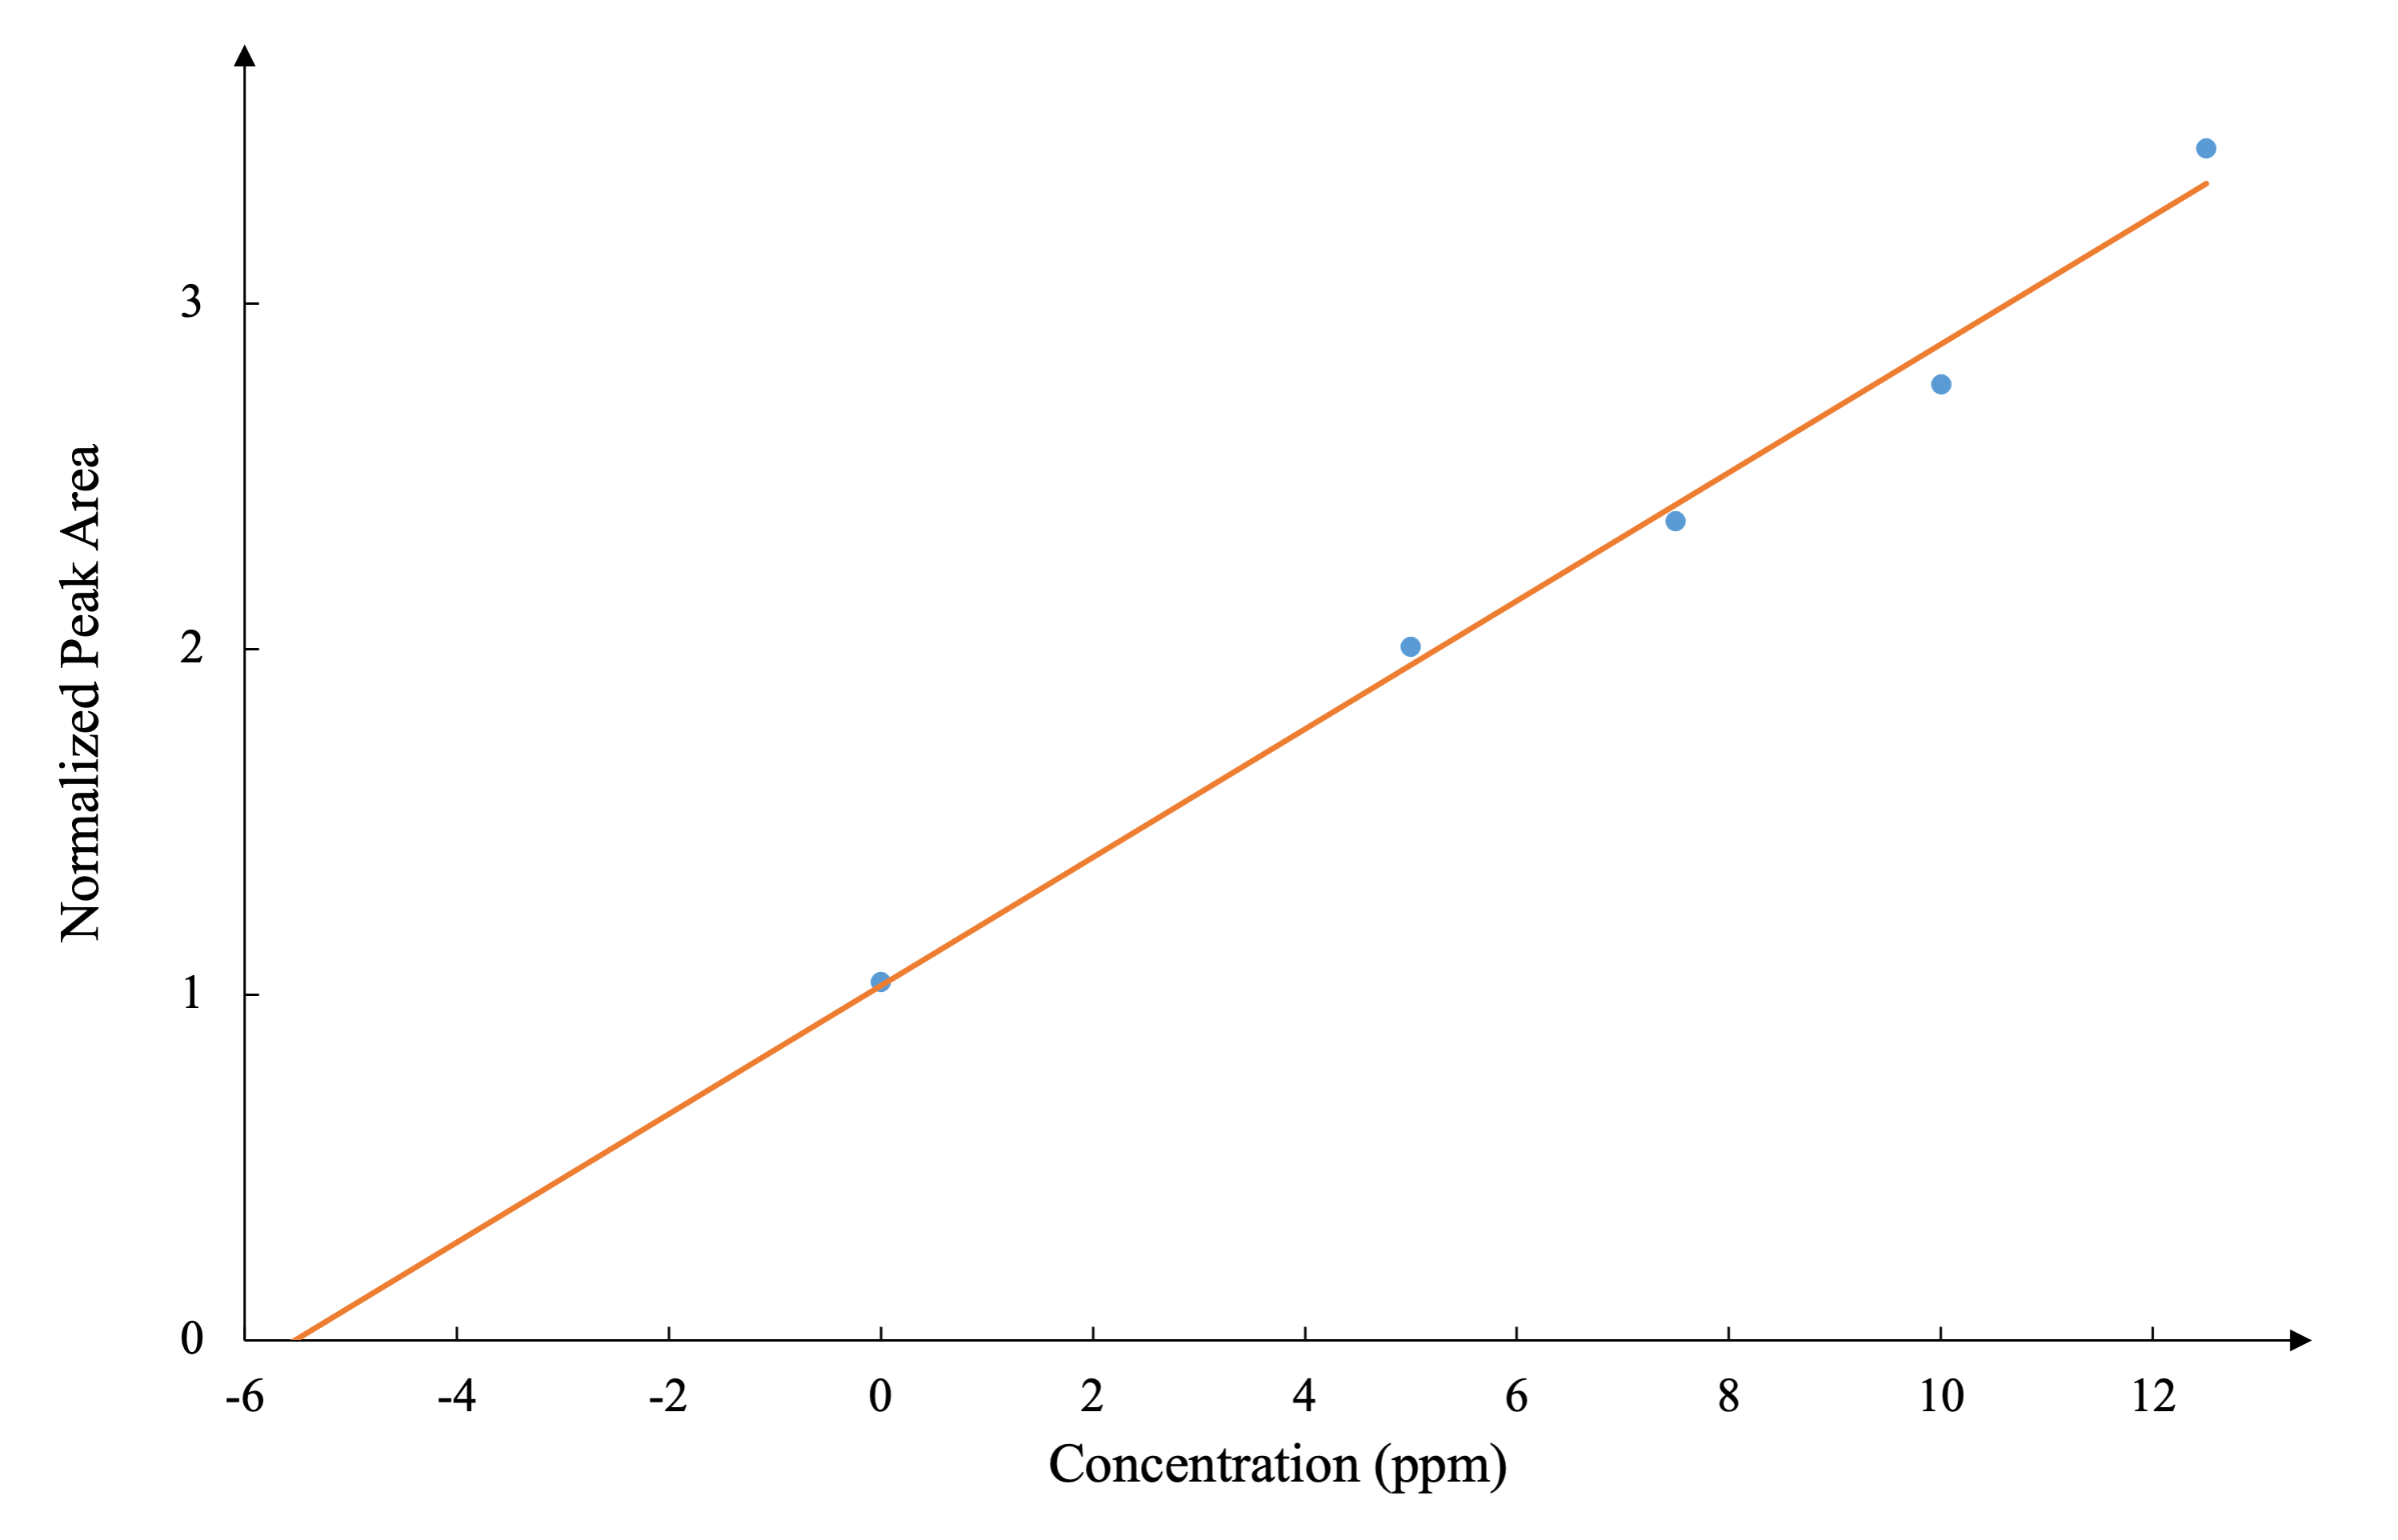
\includegraphics[width=0.95\linewidth]{lab4-StdAdd.png}
    \caption{Standard addition of benzene.}
    \label{fig:StdAdd}
\end{figure}

\begin{table}[H]
    \centering
    \small
    \renewcommand{\arraystretch}{1.2}
    \begin{tabular}{|c|c|}
        \hline
        \textbf{Concentration (v/v)} & \textbf{Error (v/v)}\\
        \hline
        \num{3.95e-4} & $\pm\num{1.66e-4}$\\
        \hline
    \end{tabular}
    \caption{Concentration of benzene in gasoline.}
    \label{tab:benzeneConcError}
\end{table}

\begin{figure}[H]
    \centering
    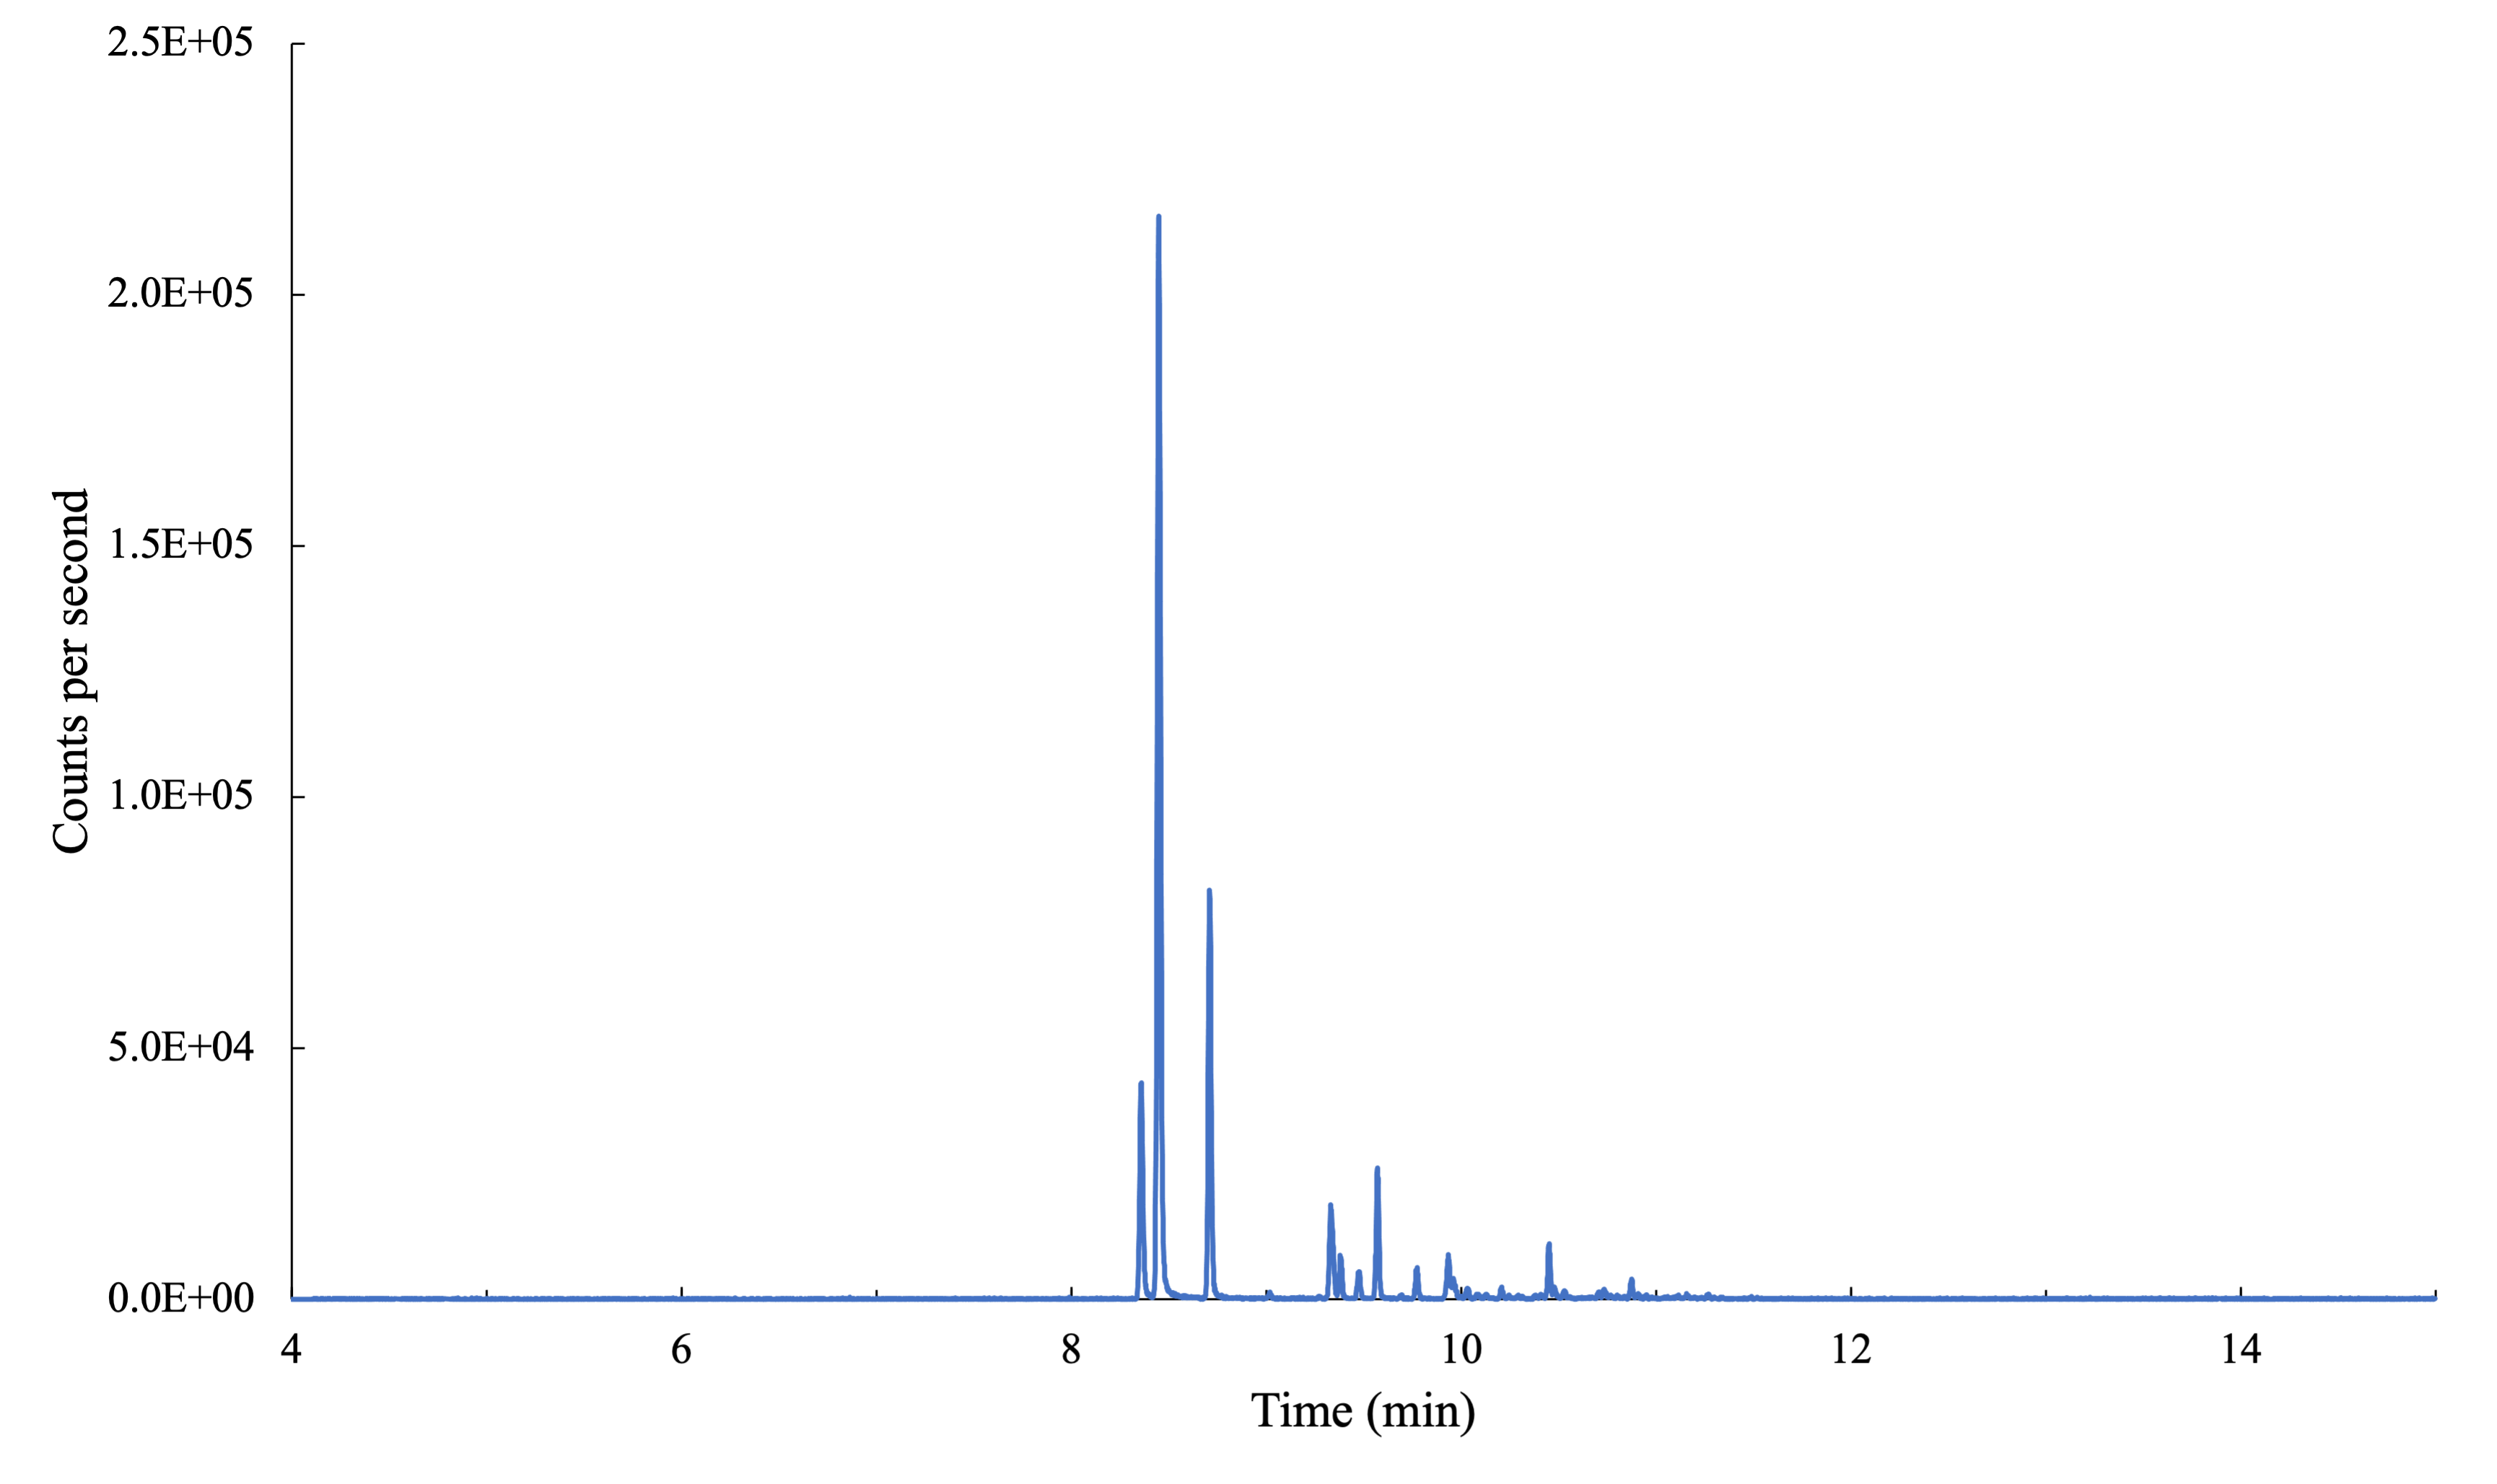
\includegraphics[width=0.95\linewidth]{lab4-EtBzEIC.png}
    \caption{Extracted ion chromatogram of ethylbenzene.}
    \label{fig:EtBzEIC}
\end{figure}

\begin{figure}[H]
    \centering
    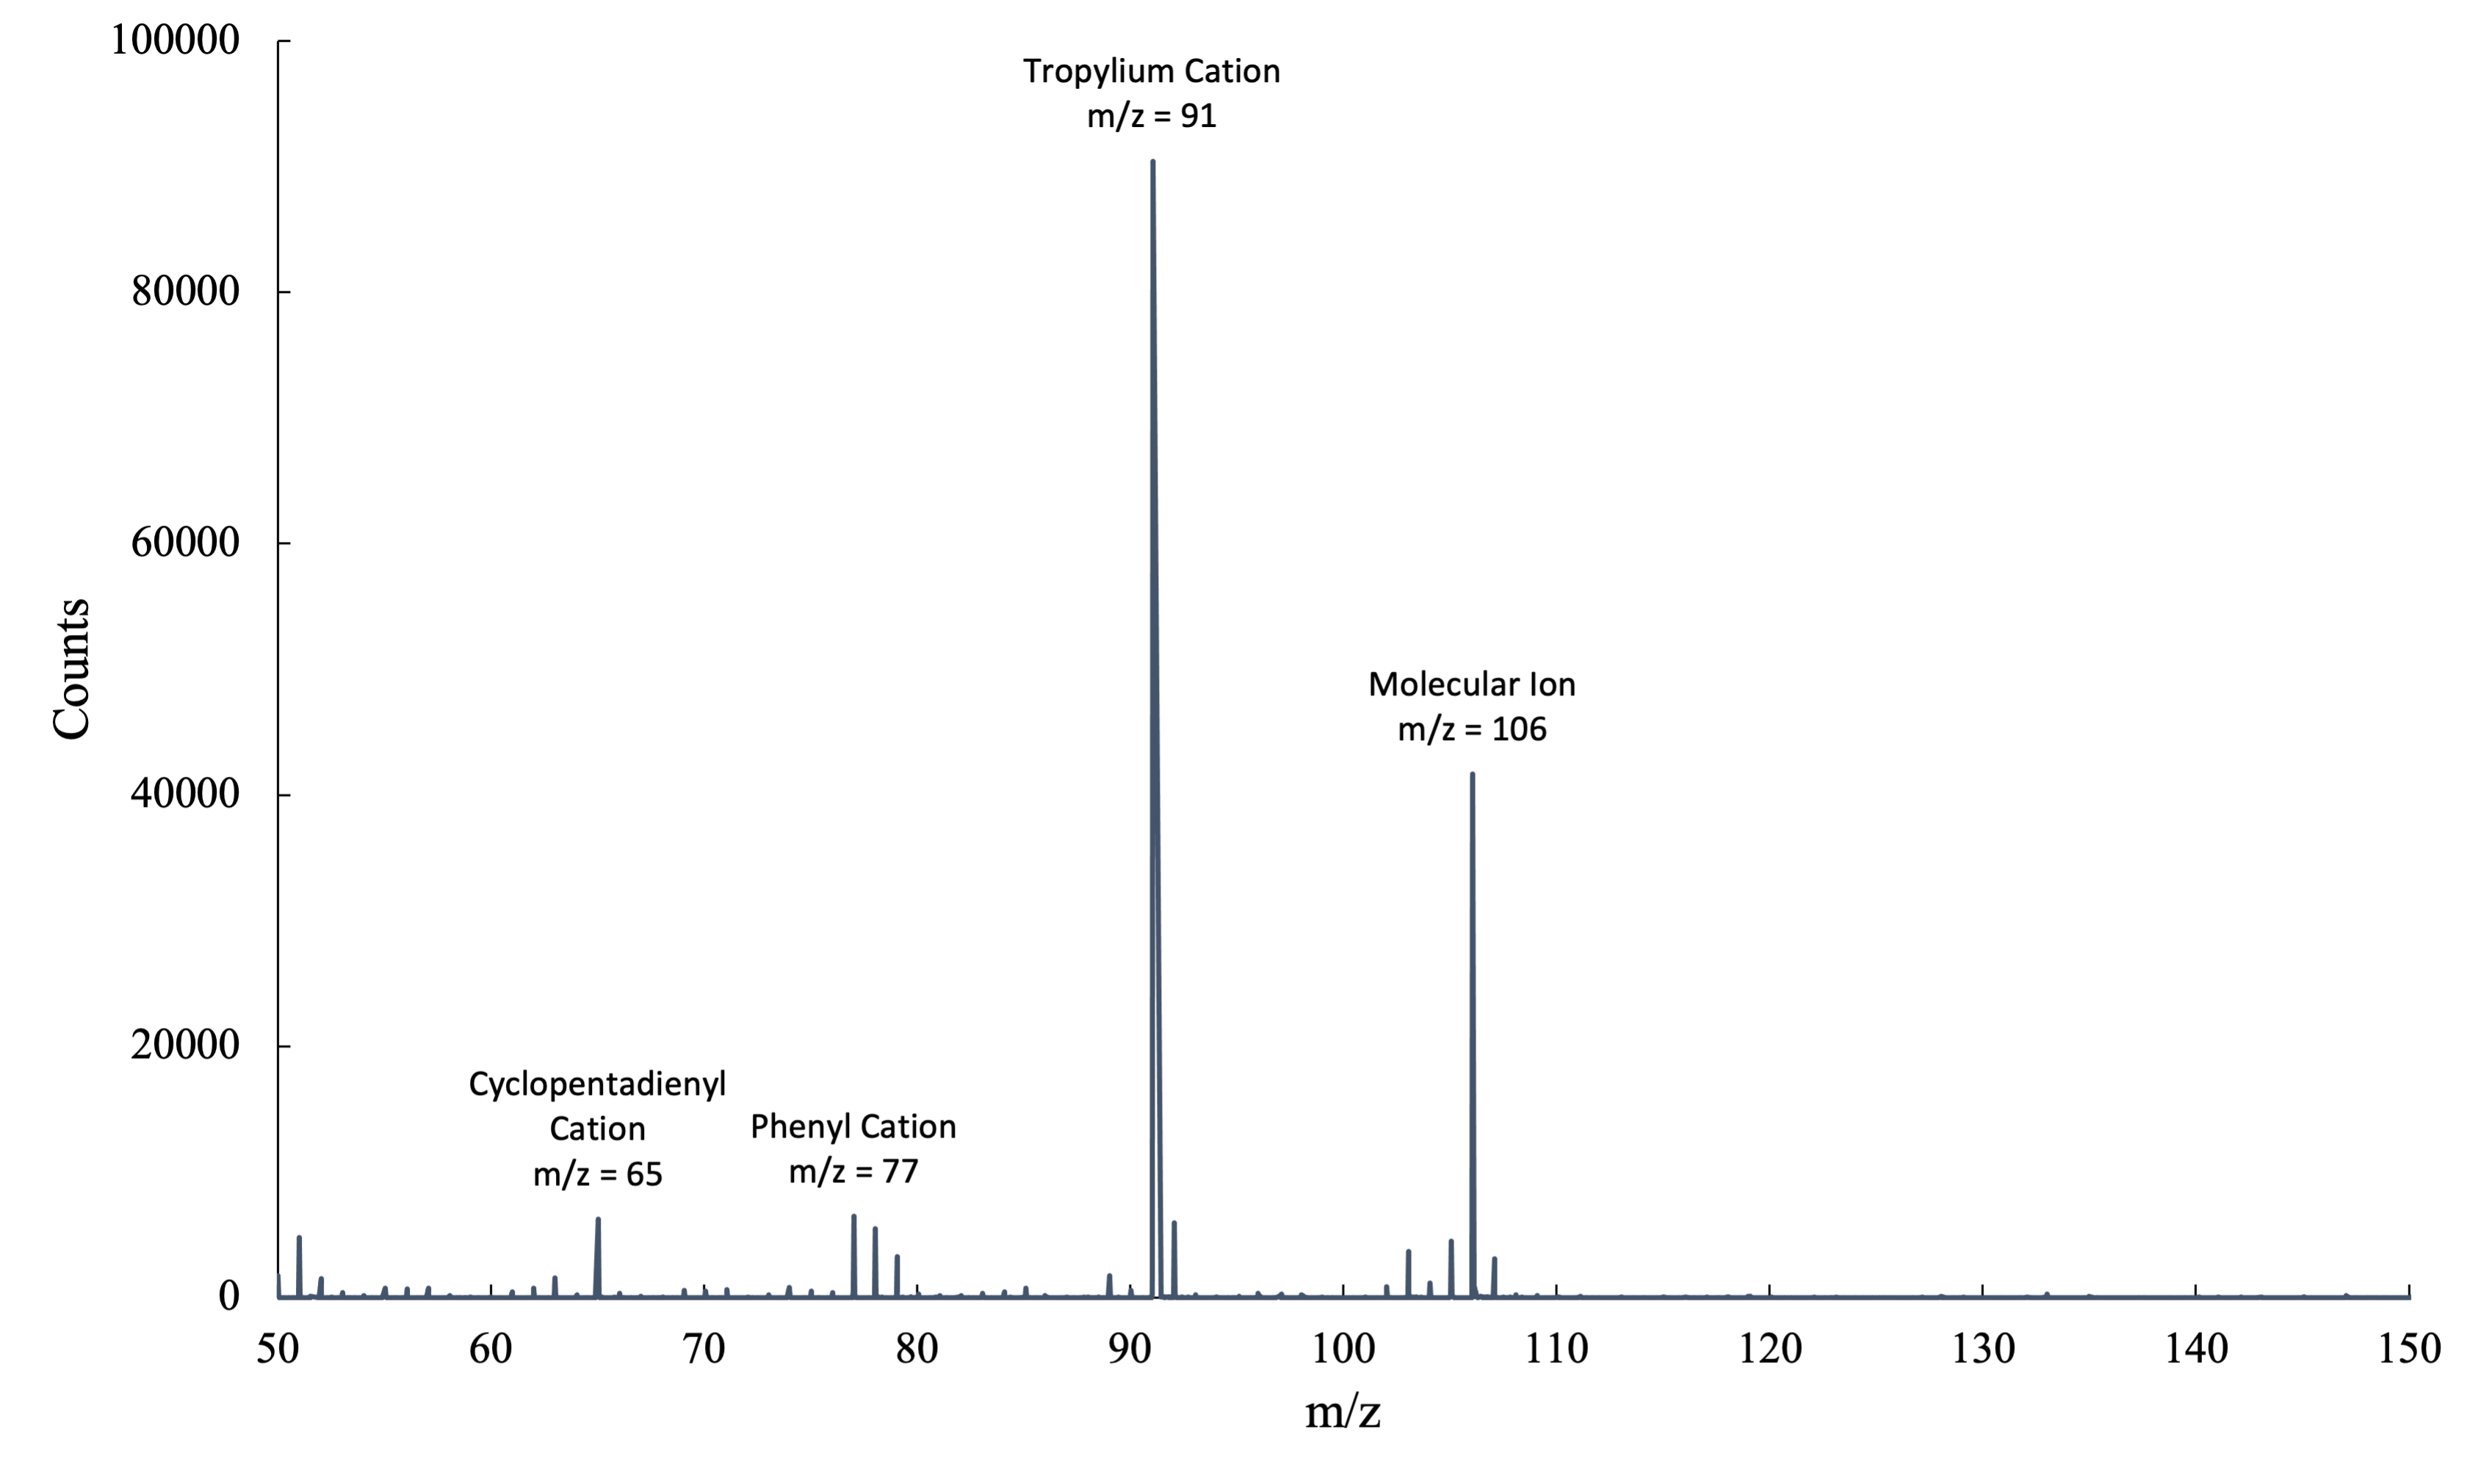
\includegraphics[width=0.95\linewidth]{lab4-EtBzMS.png}
    \caption{Extracted mass spectra of ethylbenzene.}
    \label{fig:EtBzMS}
\end{figure}

\begin{figure}[H]
    \centering
    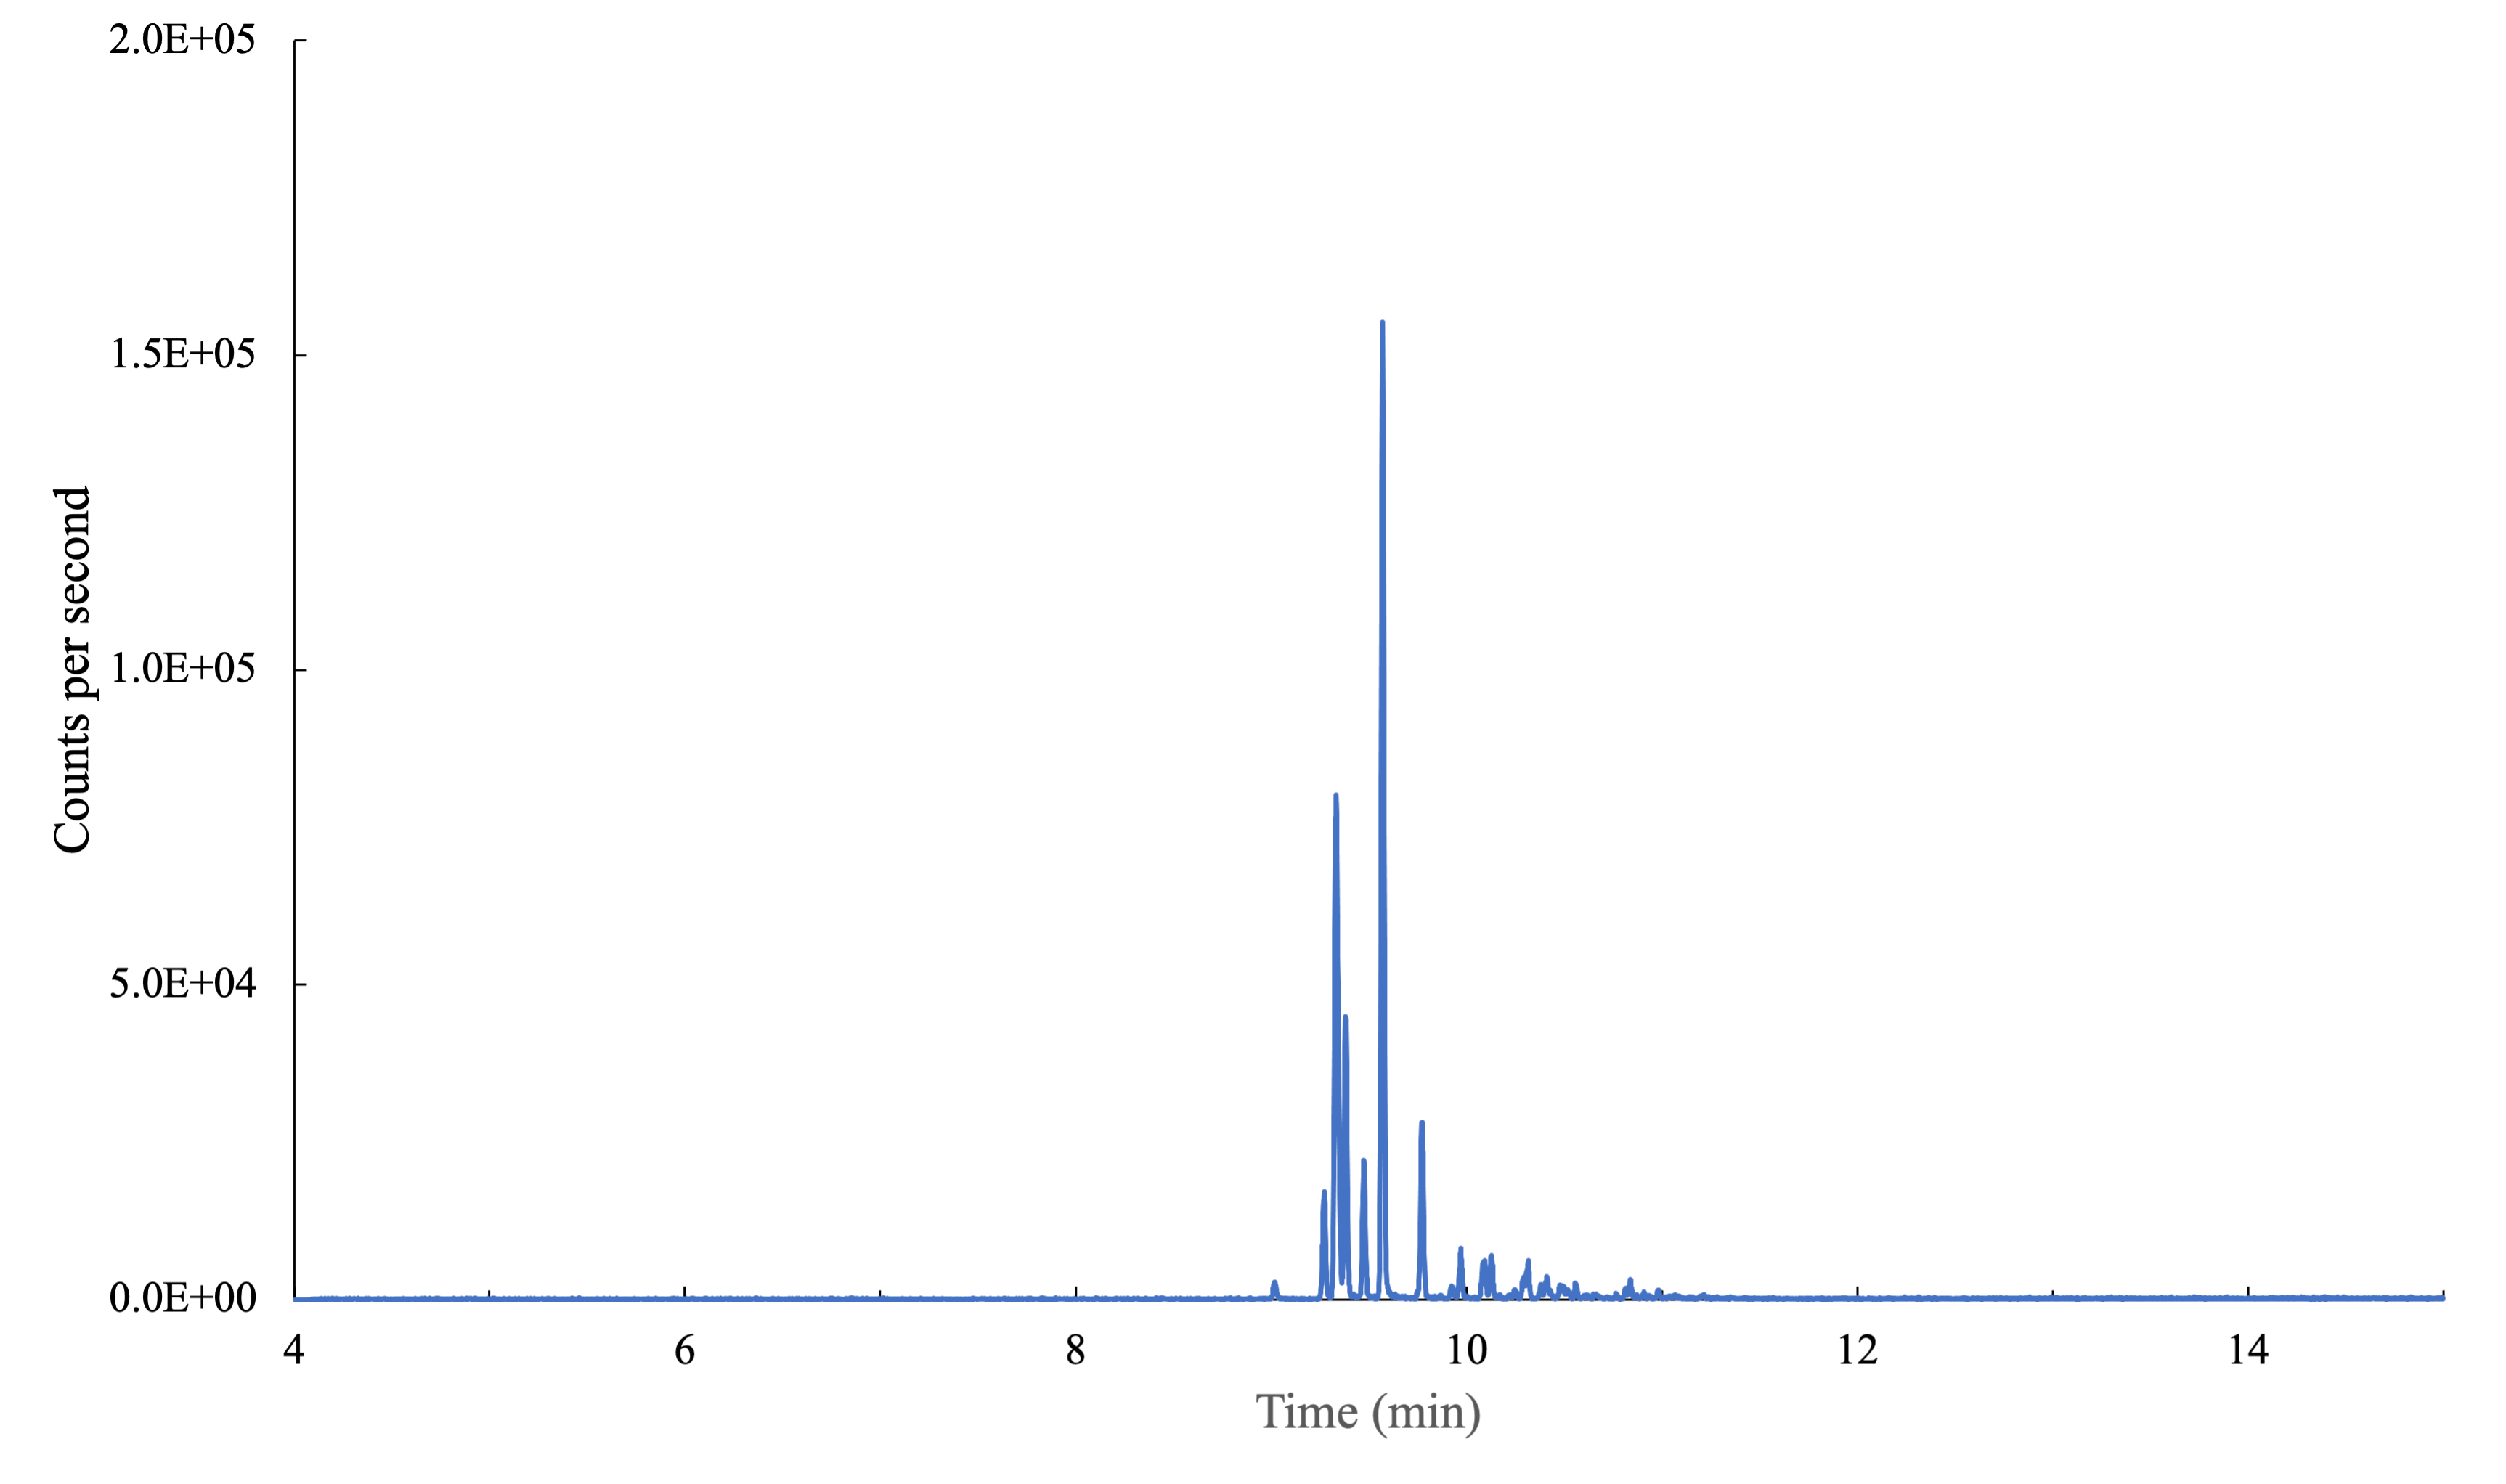
\includegraphics[width=0.95\linewidth]{lab4-mesityleneEIC.png}
    \caption{Extracted ion chromatogram of mesitylene.}
    \label{fig:mesityleneEIC}
\end{figure}

\begin{figure}[H]
    \centering
    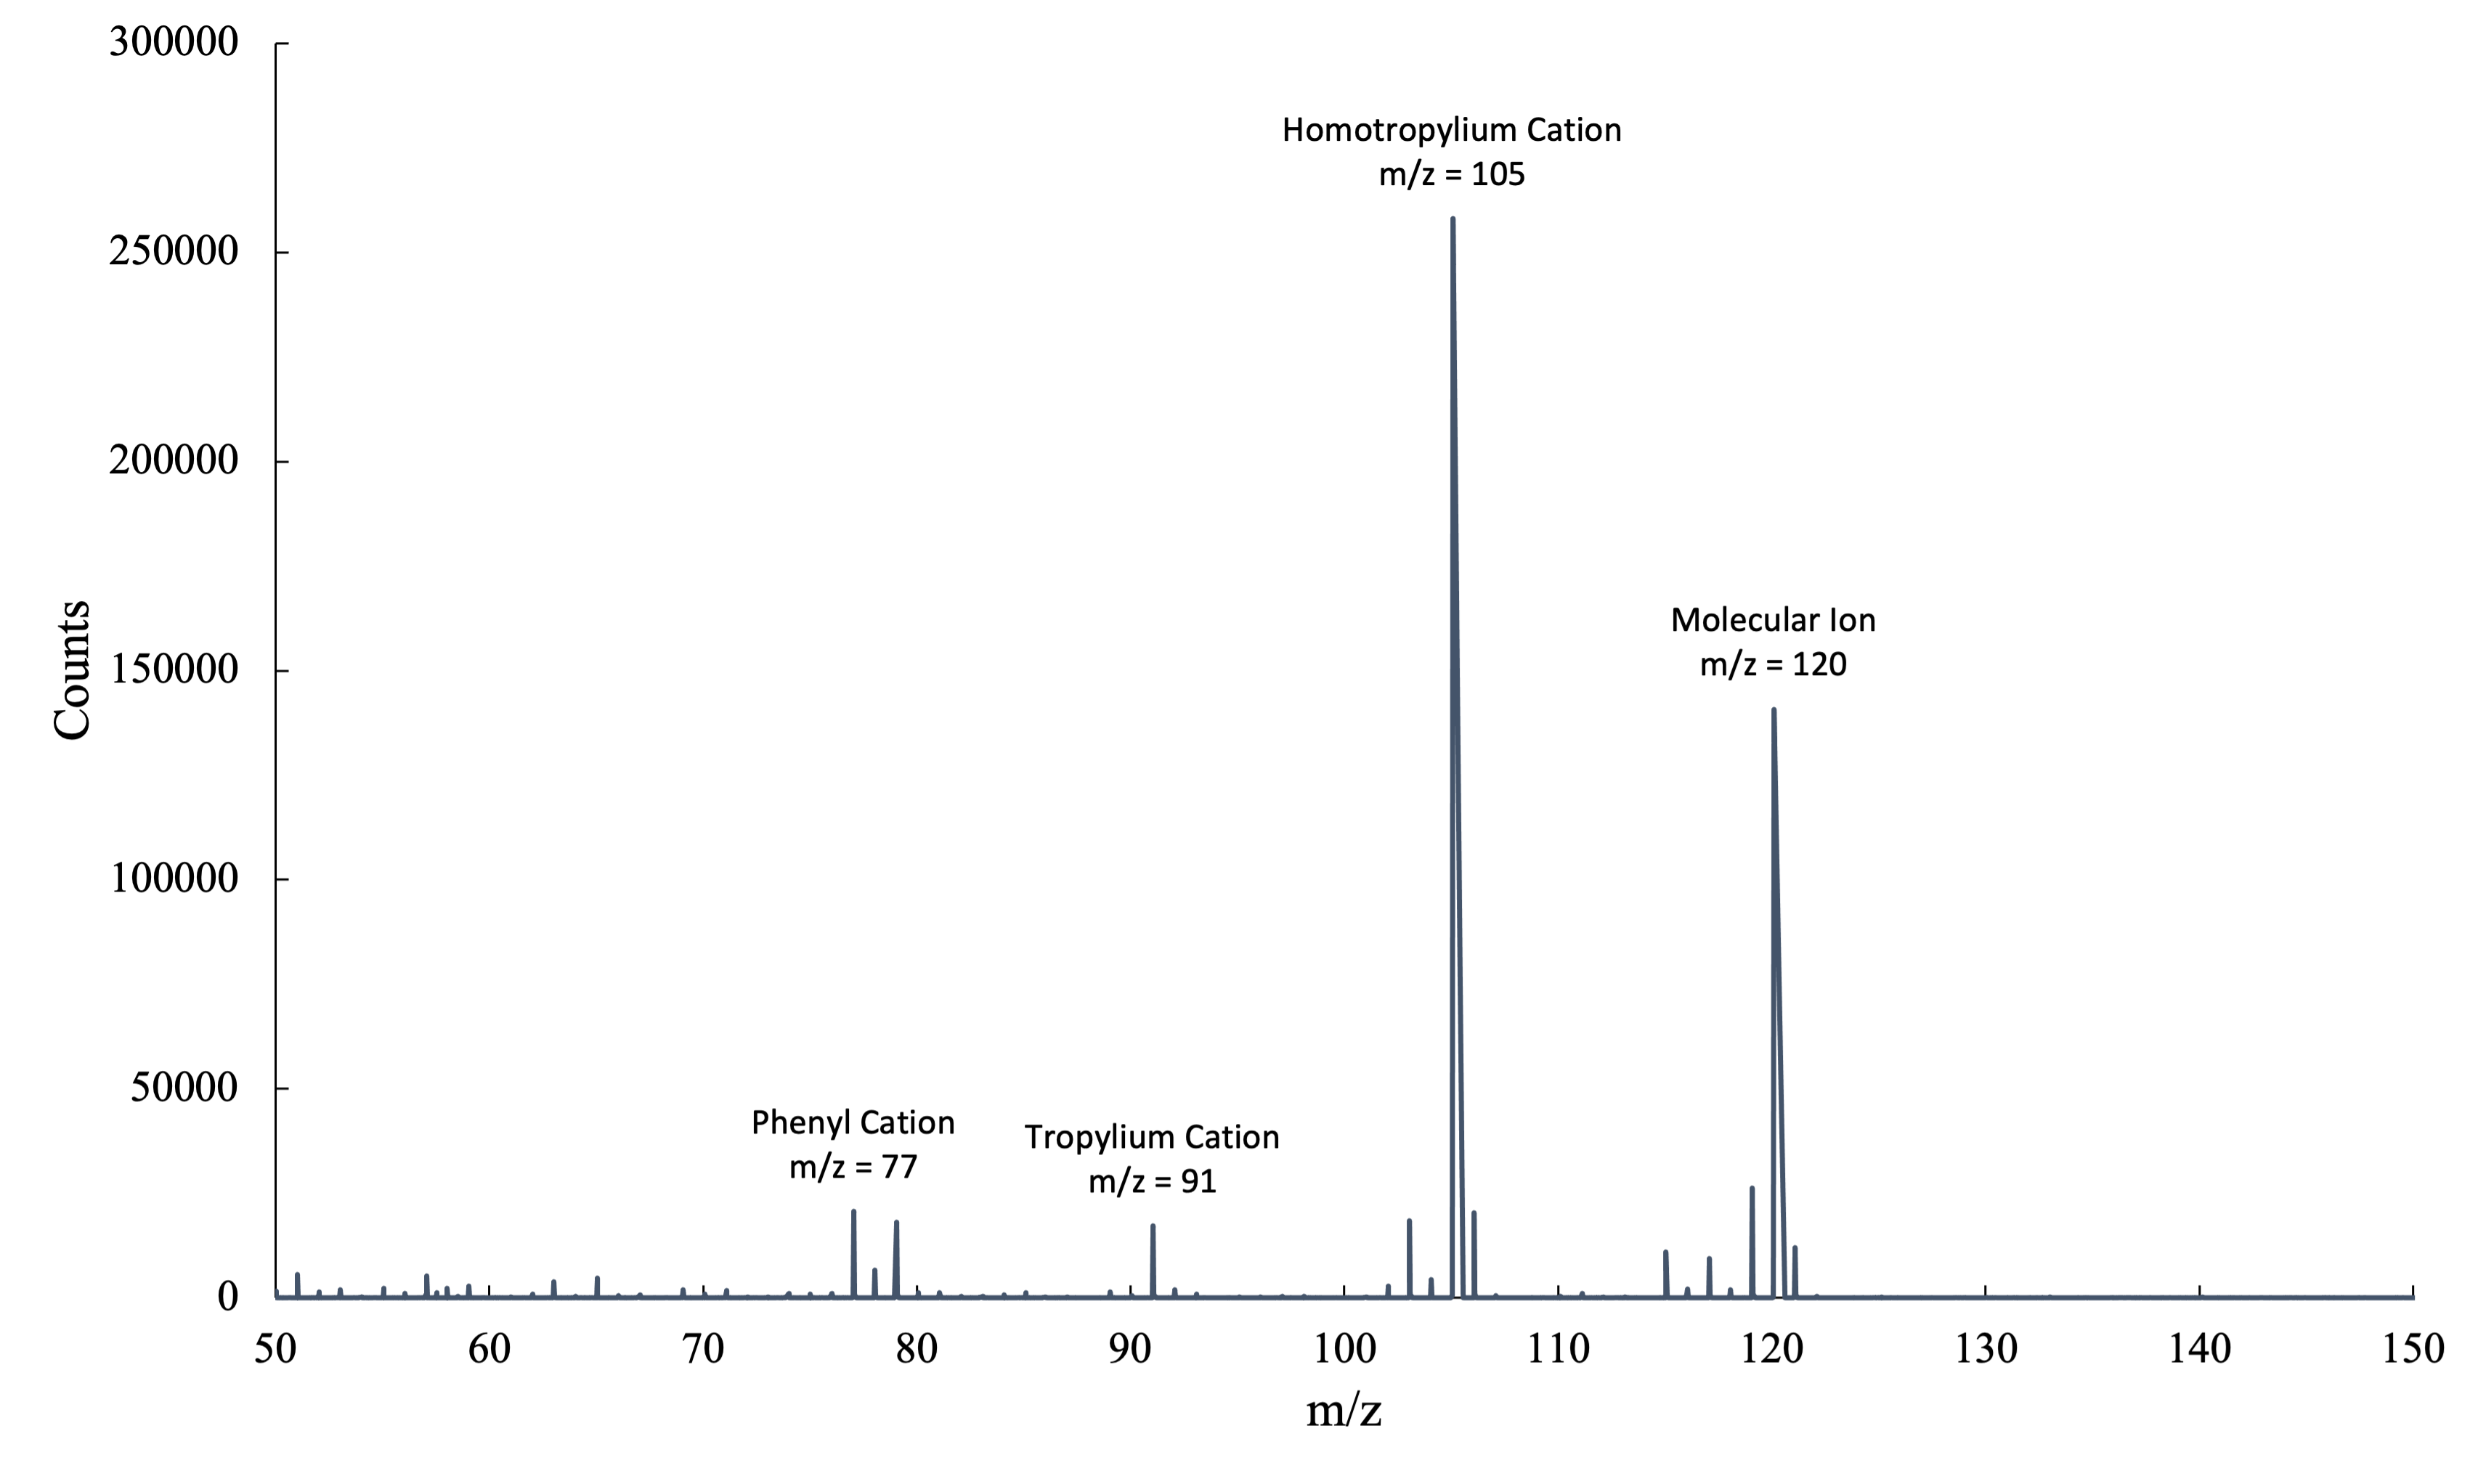
\includegraphics[width=0.95\linewidth]{lab4-mesityleneMS.png}
    \caption{Extracted mass spectra of mesitylene.}
    \label{fig:mesityleneMS}
\end{figure}

\begin{table}[H]
    \centering
    \small
    \renewcommand{\arraystretch}{1.2}
    \begin{tabular}{|c|c|c|}
        \hline
         & \textbf{Ethylbenzene} & \textbf{Mesitylene}\\
        \hline
        \textbf{Concentration (ppm)} & \num{1.71} & \num{2.48}\\
        \hline
    \end{tabular}
    \caption{Concentrations of additional aromatic molecules.}
    \label{tab:EtBzMesityleneConc}
\end{table}
These substances may not follow the same peak area-to-concentration fit as benzene (Figure \ref{fig:StdAdd}). Indeed, to more accurately determine the concentrations of these substances in gasoline, it would be appropriate to do a standard addition analysis for both of them, individually, instead of relying on more distantly related correspondences.
\setcounter{figure}{0}
\setcounter{table}{0}




\end{document}